\section{Risultati}
Vengono riportati alcuni risultati di esempio ottenuti eseguendo il programma:
\newline

Binary digits of log2 starting at position 1: 10110001

Binary digits of log2 starting at position 100: 00011111

Binary digits of log2 starting at position 10000: 00101101

Binary digits of log2 starting at position 1000000: 11010100

Binary digits of log2 starting at position 100000000: 01100111
\newline

Hexadecimal digits of pi starting at position 1: 243F6A88

Hexadecimal digits of pi starting at position 100: C29B7C97

Hexadecimal digits of pi starting at position 10000: 68AC8FCF

Hexadecimal digits of pi starting at position 1000000: 26C65E52

Hexadecimal digits of pi starting at position 10000000: 17AF5863

\subsection{Tempo di computazione}
Durante l'esecuzione del programma sul mio computer, ho ottenuto i seguenti tempi di calcolo in funzione della posizione della cifra richiesta $n$:

\begin{tikzpicture}
\begin{axis}[
    width=\textwidth,
    title={Tempo di calcolo (millisecondi)},
    xlabel={n},
    xmin=0,
    xmax=1000000,
    ymin=0,
    legend pos=north west,
    ymajorgrids=true,
    grid style=dashed,
]
 
\addplot table
  [
      color=blue,
      col sep=comma,
      trim cells=true,
    y=time,
    mark=none
    ]
    {../data/elapsed_times.pi.csv};
    \legend{$\pi$}
 
\addplot table
  [
    color=green,
    col sep=comma,
    trim cells=true,
    y=time,
    mark=none
  ]
  {../data/elapsed_times.log2.csv};
  \legend{$log(2)$}

\end{axis}
\end{tikzpicture}

\noindent Si può notare come gli algoritmi siano lineari rispetto all'input $n$.

Il peso viene dato dalle sommatorie presenti sia nel calcolo di $log(2)$ che per $\pi$, in entrambi i casi hanno $O(n)$ termini.
\newline

Come intuibile, si vede anche come il calcolo per $log(2)$ sia meno costoso rispetto a quello per $\pi$. 

\subsection{Possibili (futuri) utilizzi}
Partendo dal fatto che le cifre in $\pi$ \textbf{sembrano}\footnote{Non è stato dimostrato per il momento.} comparire equiprobabilmente, si potrebbe dedurre che prima o poi sia possibile incontrare qualunque sequenza di cifre.

Per questo motivo si può pensare di codificare un file, che non è altro che una sequenza di cifre, \textit{all'interno} di $\pi$.
Sarebbe sufficiente memorizzare solo la posizione della cifra iniziale e la sua lunghezza. Recuperarlo in seguito usando il calcolo dell'n-sima cifra sarebbe \textit{relativamente facile}.

\noindent Sebbene per il momento il calcolo richiederebbe troppo tempo, rendendo questa tecnica inutilizzabile, il grafico che segue mostra i dati ottenuti sulla frequenza di comparsa delle singole cifre all'interno del primo milione di cifre:
\newline \newline
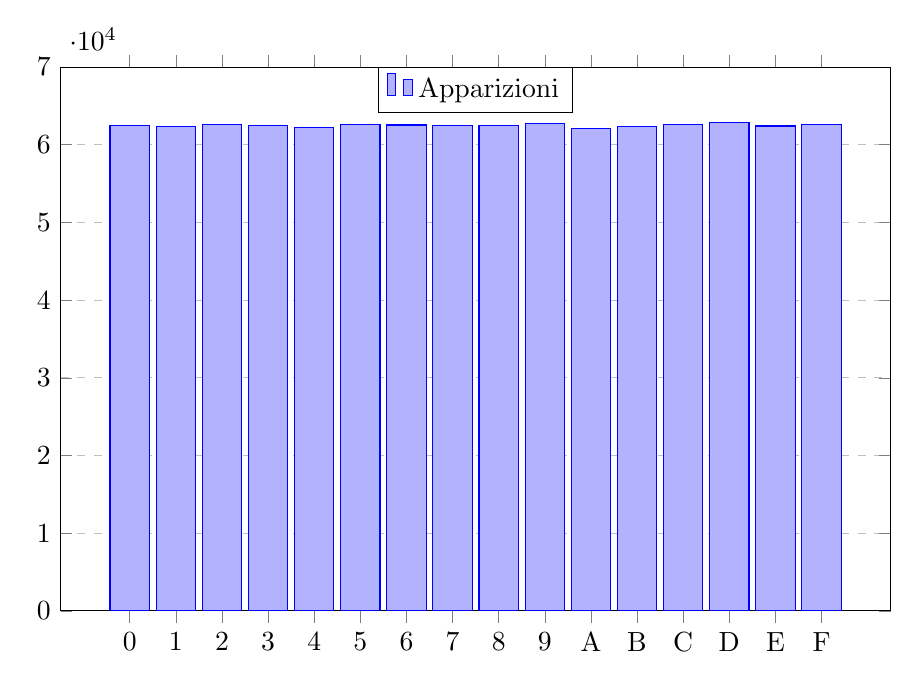
\begin{tikzpicture}
\begin{axis}[
  ybar,
  bar width=.5cm,
  width=\textwidth,
  height=.70\textwidth,
  ymin=0, ymax=70000,
  ymajorgrids=true,
  grid style=dashed,
  symbolic x coords={0,1,2,3,4,5,6,7,8,9,A,B,C,D,E,F},
  xtick=data,
  legend style={at={(0.5,1)},
  anchor=north,legend columns=-1},
]
\addplot 
  coordinates {(0,62522) (1,62385) (2,62644) (3,62432) (4,62235) (5,62649) (6,62545) (7,62515) (8,62459) (9,62699) (A,62070) (B,62345) (C,62621) (D,62829) (E,62415) (F,62635)};
  \legend{Apparizioni}
\end{axis}
\end{tikzpicture}

Risulta evidente che ogni cifra appare più o meno la stessa quantità di volte delle altre. Questo potrebbe aprire nuove strade sull'utilizzo di costanti come il Pi greco per la codifica e compressione di file.